\section{Implementation}

\subsection[The simple case]{The simple case}
\begin{frame}
\frametitle{The simple case}

\begin{itemize}
	\item Trivial cases (simple expresions)
	\begin{itemize}
		\item Not so trivial
		\item Meaningful messages
	\end{itemize}
\end{itemize}

\begin{center}
\begin{tabular}{ c c }
  	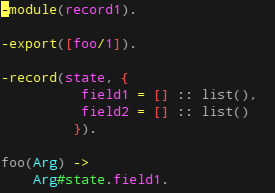
\includegraphics[scale=0.45]{../figures/test1}
&
  	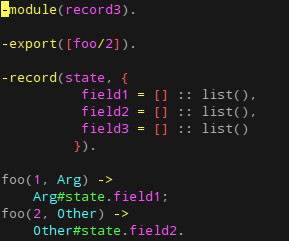
\includegraphics[scale=0.45]{../figures/test2}
\end{tabular}
\end{center}

\end{frame}

\begin{frame}
\frametitle{Non trivial cases}

\begin{itemize}
	\item Escape cases
	\begin{itemize}
		\item Replicate
		\item Return
		\item Call
	\end{itemize}
\end{itemize}

\begin{center}
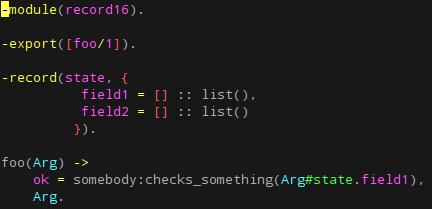
\includegraphics[scale=0.45]{../figures/test16}
\end{center}
\end{frame}

\begin{frame}
\frametitle{Extending to cover the whole language}

\begin{columns}
\begin{column}[l]{3.5cm}

	\begin{block}{}
		\begin{itemize}
			\item \scriptsize{comparisons}
			\item \scriptsize{switches}
			\item \scriptsize{guards}
		\end{itemize}
	\end{block}

	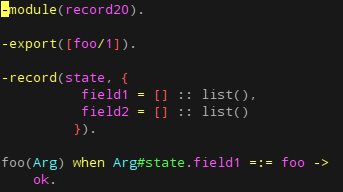
\includegraphics[scale=0.4]{../figures/test20}

\end{column}

\begin{column}[r]{4.5cm}
\begin{tabular}{ c }
  	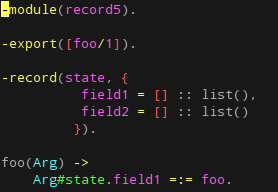
\includegraphics[scale=0.4]{../figures/test5}
\\
	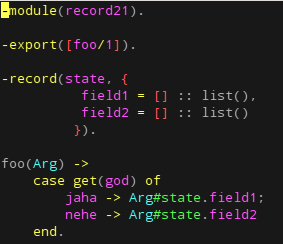
\includegraphics[scale=0.4]{../figures/test21}
\end{tabular}
\end{column}
\end{columns}

\end{frame}

\begin{frame}
\frametitle{Simulating real bugs}

\begin{center}
\begin{tabular}{ c c }
  	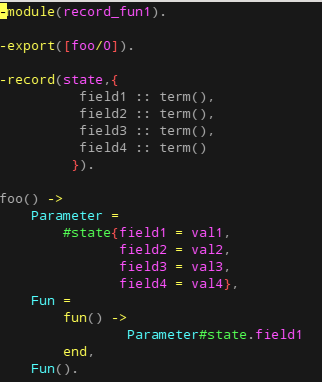
\includegraphics[scale=0.4]{../figures/rec_fun1}
&
	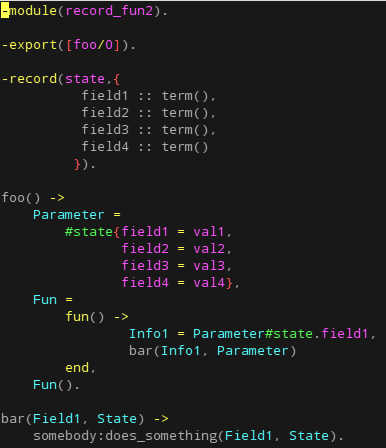
\includegraphics[scale=0.4]{../figures/rec_fun2}
\end{tabular}
\end{center}
\end{frame}